\chapter{Fundamentação Teórica}
\label{c.fundamentacao}

\section{Realidade Virtual}
\label{s.rv}
A realidade virtual “é uma interface avançada para aplicações computacionais, que permite ao usuário a movimentação (navegação) e interação em tempo real, em um ambiente tridimensional, podendo fazer uso de dispositivos multissensoriais, para atuação ou \textit{feedback}.” \cite[p. ~7]{torilivro}

A tecnologia de RV permite a imersão do usuário em um ambiente virtual através de um sistema computacional. Com esta tecnologia, é possível enganar os sentidos do usuário para que o mesmo tenha a sensação de que está dentro do ambiente simulado. 

É importante diferenciar os conceitos de RV, realidade aumentada (RA) e virtualidade aumentada (VA). Como explica \citeonline{milgram}, o ambiente propiciado pela RV é totalmente sintético, ou virtual, e pode ou não imitar o mundo real. Já ambientes em RA intercalam o real e o virtual tornando o capacete de visualização “transparente”, acrescentando elementos virtuais no ambiente real. Por fim, a VA traz ambientes virtuais com alguns elementos reais como a representação das mãos do usuário, por exemplo. A Figura ~\ref{f.milgram} mostra uma relação entre as tecnologias descritas acima.

\begin{figure}[ht]
	\caption{\small \textit{Virtual Reality Continuum}}
	\centering
	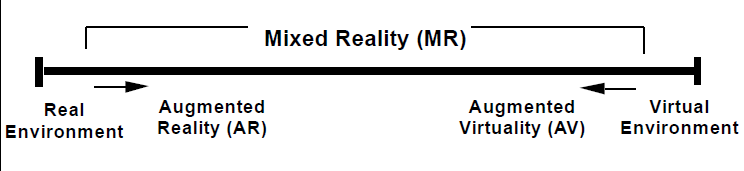
\includegraphics[scale=0.7]{Imagens/milgram.png}
	\label{f.milgram}
	\legend{\small Fonte: \cite{milgram}}
\end{figure}

Para se criar a sensação de imersão propiciada pela RV, é utilizada a estereoscopia (Figura ~\ref{f.estereoscopia}), ou seja, é gerada uma imagem para cada olho. Esta técnica faz com que o cérebro interprete as imagens como uma. \citeonline[p. ~221]{siscoutto} explicam que a importância da estereoscopia ou visão binocular pode ser averiguada na prática ao fechar um olho e tentar exercer atividades cotidianas desta forma. O que será observado é que a visão monocular, torna o simples ato de pegar um objeto sobre a mesa uma tarefa difícil pois esta visão conta com uma percepção rudimentar de profundidade.

\begin{figure}[H]
	\caption{\small Estereoscopia}
	\centering
	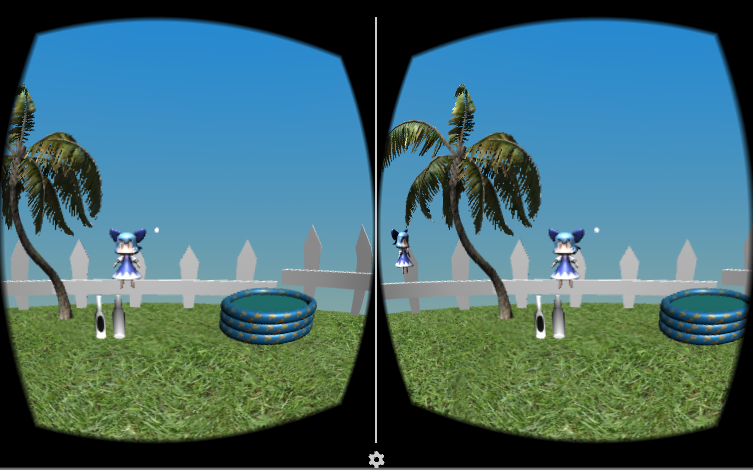
\includegraphics[scale=0.7]{Imagens/estereoscopia.png}
	\label{f.estereoscopia}
	\legend{\small Fonte: Elaborada pelo autor.}
\end{figure}

Além da estereoscopia, a navegação e a interação com o ambiente virtual também são características da RV. De acordo com \citeonline[p. ~9]{torilivro}, a navegação em espaços tridimensionais dá-se por movimentos de translação e de rotação ao longo dos três eixos (X, Y, Z) resultando em 6 graus de liberdade (3 de rotação e 3 de translação) como mostra a Figura ~\ref{f.grausliberdade}. 

\begin{figure}[ht]
	\caption{\small Graus de Liberdade}
	\centering
	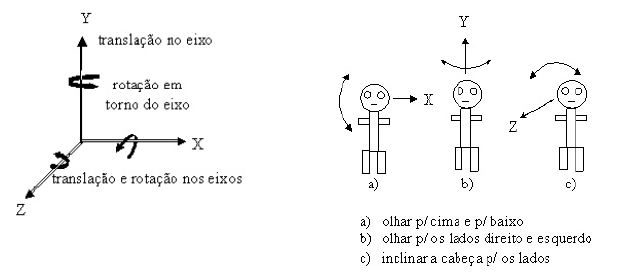
\includegraphics[scale=1.0]{Imagens/grausliberdade.png}
	\label{f.grausliberdade}
	\legend{\small Fonte: \cite{torilivro}.}
\end{figure}

O conceito de realidade virtual, segundo \citeonline[p. ~98]{rodrigues}, apesar de existir a mais de vinte anos, alcançou popularidade apenas recentemente. Este fato se deu devido a diminuição do custo para a sua implementação.

\subsection{Fatores Fisiológicos}
\label{ss.fatoresfisiologicos}
Quando tenta-se criar uma simulação imersiva, é importante ter em mente alguns fatores fisiológicos que não são levados em consideração em aplicações não imersivas. Estes fatores, quando não implementados corretamente, podem levar ao chamado \textit{motion sickness} ou VR \textit{sickness} que, segundo a \citeonline{vrsickness}, é a sensação de náusea devido à disparidade entre o que é sentido e o que é esperado sentir. Esta disparidade faz com que nosso corpo se sinta “envenenado” causando desconforto ao usuário. 

De acordo com a \citeonline{oculus}, encontrar fatores que contribuem para o \textit{motion sickness} pode ser complicado pois as pessoas sentem este desconforto de forma desigual. Enquanto um pode sentir náusea em um curto período de exposição à uma aplicação em RV, outro pode não sentir nada após um longo período. Outro empecilho é a possibilidade de se acostumar ao ambiente imersivo e não sentir mais o desconforto. Por isso, não é recomendado que os desenvolvedores da aplicação determinem quais são ou não fatores causadores do VR \textit{sickness}. 

Como alternativa, é recomendado evitar algumas características que, segundo a \citeonline{oculus} demonstraram serem fatores contribuintes para o desconforto do usuário. Um destes fatores é a aceleração da câmera. Diferente de aplicações não imersivas, a movimentação do usuário pela aplicação deve ser analisada com cuidado pois, como o usuário está parado enquanto o personagem está se movimentando, ocorre a discrepância de sensações resultando no desconforto.

Outro fator é o grau de controle do usuário sobre o ambiente. Ao travar a tela para que alguma mensagem seja visualizada ou realizar a rotação da câmera para algum ponto, é retirado o poder de controle do usuário, o que também é considerado um fator facilitador do VR \textit{sickness}.

A distância dos objetos à câmera também deve ser analisada. O usuário deve ser capaz de ler uma mensagem em frente à câmera com facilidade, o posicionamento incorreto da mensagem pode causar incômodo ao usuário dificultando a leitura.

Tendo em vista a redução do VR \textit{sickness} foram criados guias de boas práticas para serem levados em consideração ao desenvolver aplicações em RV.

\subsection{Boas Práticas}
\label{ss.boaspraticas}

Para auxiliar desenvolvedores, a Google® lançou um aplicativo para dispositivos Android denominado \textit{Cardboard Design Lab} (Figura ~\ref{f.designlab}). Neste aplicativo, o usuário pode aprender técnicas que são classificadas em duas categorias: criação e imersão. A primeira categoria, segundo \citeonline{hopkins}, foca nos princípios básicos da criação de aplicações em RV. Já a segunda categoria é mais exploratória, levando em consideração teoria e experiências através do aplicativo. Em cada categoria são fornecidas lições onde o usuário verá cenários onde as técnicas são aplicadas e, em alguns casos, sentirá o \textit{motion sickness} quando determinado cuidado não for tomado. 

\begin{figure}[H]
	\caption{\small Cardboard Design Lab}
	\centering
	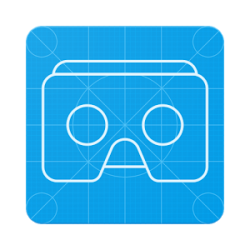
\includegraphics[scale=0.5]{Imagens/designlab.png}
	\label{f.designlab}
	\legend{\small Fonte: \cite{designlab}}
\end{figure}

Primeiramente, o aplicativo mostra a necessidade de se utilizar o retículo - círculo no centro da tela que aumenta o seu raio ao passar por algum objeto, variando o seu posicionamento com base na movimentação de cabeça do usuário. Como ainda não existe o rastreamento do olho do usuário em aplicações de RV para dispositivos móveis, é muito difícil saber para onde a cabeça está apontando quando o retículo é inexistente, tornando a seleção de objetos em um cenário muito mais complicada. 

A distância entre o usuário e caixas de textos que eventualmente aparecem na tela é outro fator a ser levado em consideração. Segundo ainda o guia, uma distância confortável para a leitura é de três metros à frente da câmera. 

A movimentação do usuário no cenário pode ser feita de algumas maneiras para que não se cause o desconforto. Um modo é mover a câmera de forma constante, sem variações de aceleração. Também é possível realizar o desvanecer ou \textit{fade} da tela, que é quando a imagem do cenário desaparece e outro cenário reaparece. Segundo \citeonline{tom}, se este clique da tela estiver na frequência correta, o nosso cérebro interpreta esta mudança como um piscar dos olhos, tornando a transição imperceptível. 

Como um dos principais conceitos da realidade virtual é a imersão do usuário, o mesmo deve se sentir confortável no ambiente e, para que isso ocorra, a escala dos objetos no ambiente imersivo deve corresponder ao máximo a realidade, para que o usuário se sinta no mesmo “mundo” do espaço virtual. O mesmo vale para os sons presentes na aplicação, que devem considerar o posicionamento do usuário. Além disso, utilizar pontos de referência no ambiente evitam que o usuário se sinta desorientado. Quanto ao controle do usuário, uma recomendação geral é nunca travar a cena. Ou seja, é importante que a movimentação da cabeça esteja sempre habilitada.

Para auxiliar o usuário a navegar através da aplicação, pode-se utilizar recursos como pontos de luz para indicar o caminho a ser seguido, além de sinalizações para indicar onde o usuário deveria olhar. A última recomendação do aplicativo apresentado pela Google® é criar aplicações visualmente agradáveis como na Figura ~\ref{f.makeitbeatiful} a fim de maximizar a ilusão de imersão do usuário. 

\begin{figure}[h]
	\caption{\small Visual Agradável}
	\centering
	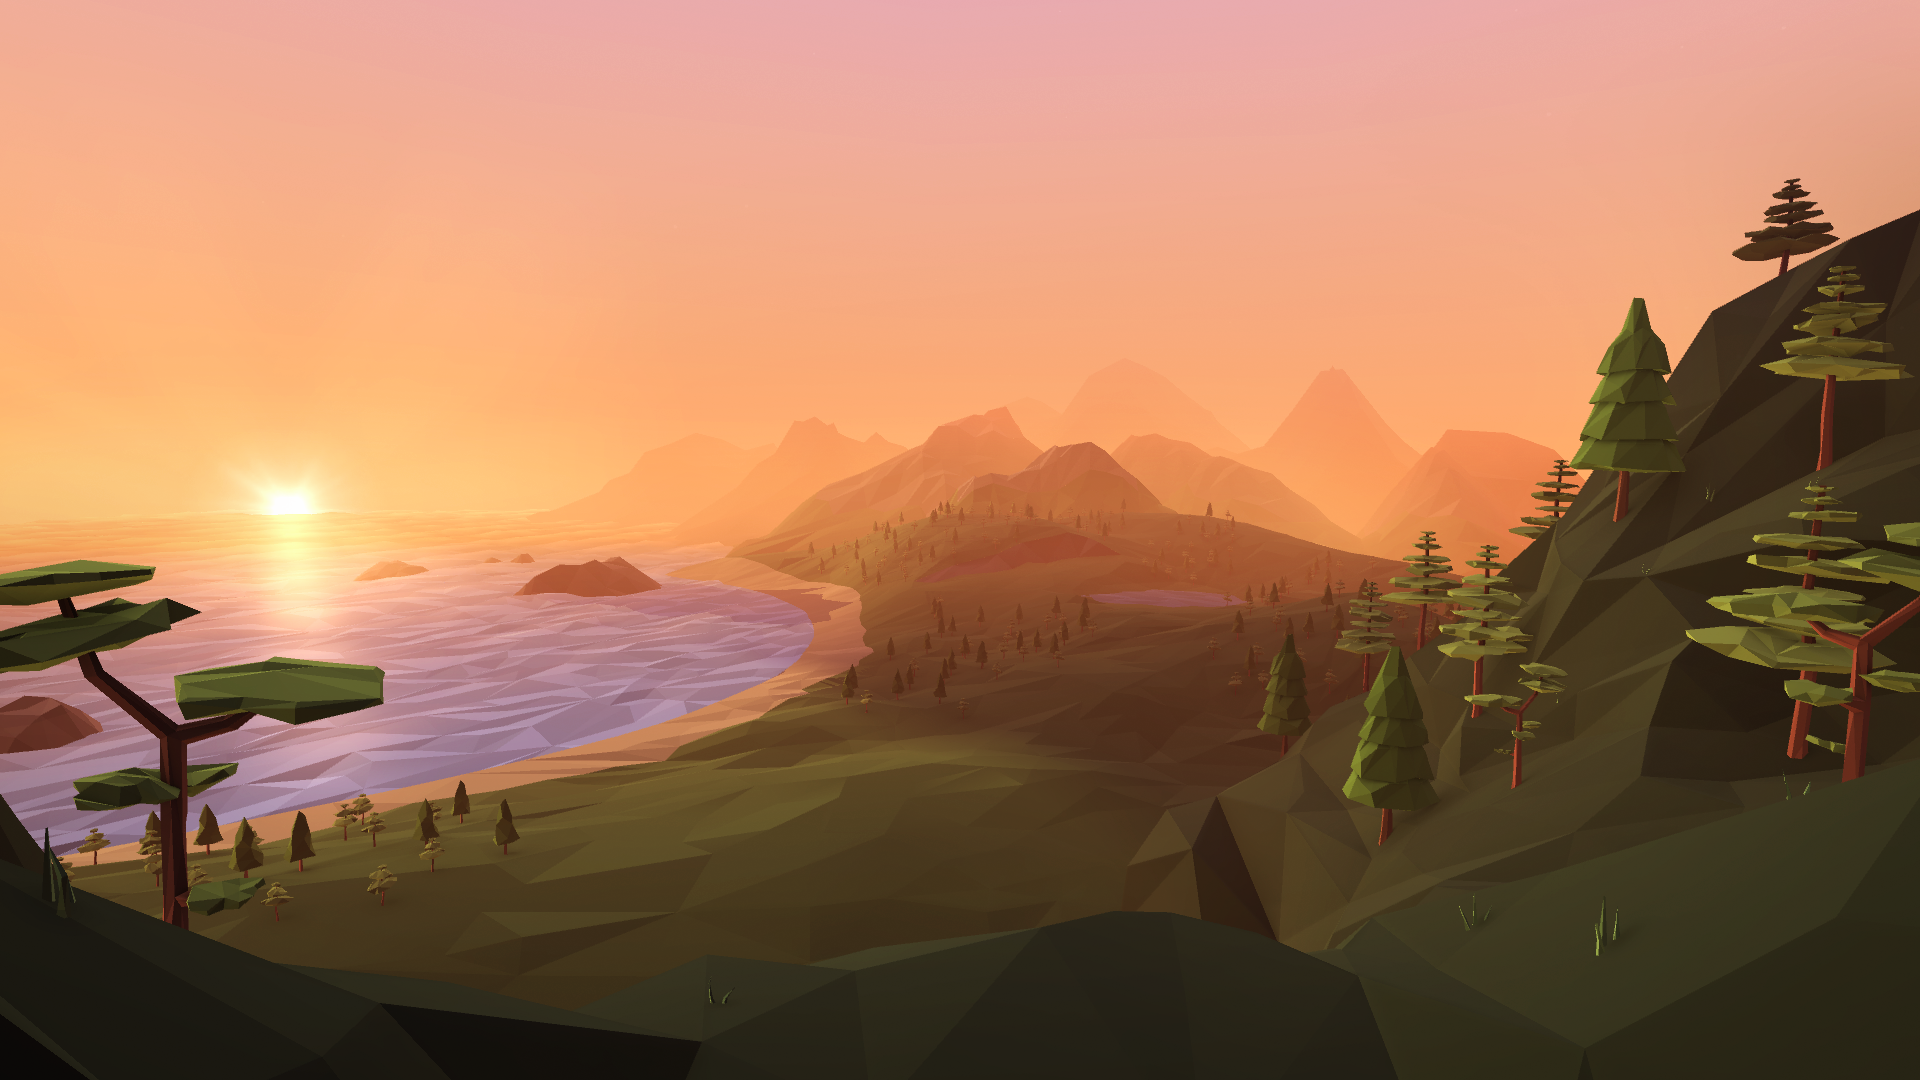
\includegraphics[scale=0.2]{Imagens/makeitbeautiful.png}
	\label{f.makeitbeatiful}
	\legend{\small Fonte: \cite{hopkins}.}
\end{figure}


\section{Dispositivos de Controle de Interação Homem/Máquina}
\label{s.dispositivos}

Com a inserção das máquinas no cotidiano das pessoas, surgiu uma área de estudos multidisciplinar que visa compreender as interações entre o usuário e o computador denominada \textit{Human Computer Interaction} (Interação Humano-Computador). Segundo \citeonline[p. ~3]{dix}, entende-se por usuário um indivíduo ou grupo de pessoas trabalhando juntas ou uma sequência de usuários em uma organização. O usuário é qualquer um que está tentando cumprir um objetivo utilizando a tecnologia. O computador representa qualquer tecnologia inclusive partes não computadorizadas como outras pessoas. Por interação entende-se qualquer meio de comunicação entre o usuário e a máquina.  

Em relação a área de estudo Interação Humano-Computador, é possível citar um grande número de dispositivos que podem ser considerados computador pelos quais o usuário irá interagir a fim de realizar algum objetivo. Como exemplos, existem os dispositivos de entrada como dispositivos de texto, de posicionamento e indicação e os dispositivos de saída como a tela do computador ou celular. 

O teclado é um dos dispositivos de entrada de texto mais comuns. De acordo com \citeonline{dix}, os teclados funcionam com o pressionar das teclas, fechando a conexão e fazendo com que um código de caractere seja enviado ao computador. Atualmente, a maioria dos teclados seguem o layout de teclas QWERT (Figura ~\ref{f.qwert}) que, apesar de não ser considerada a distribuição ótima, foi implementado pois o teclado baseou-se nas máquinas de escrever onde o posicionamento das teclas levava em consideração letras que possivelmente seriam combinadas. Estas eram colocadas distantes no teclado para se evitar que os braços se aglomerassem de um lado da máquina. Reconhecedor de voz e de escrita também podem ser considerados dispositivos de entrada de texto.

\begin{figure}[H]
	\caption{\small Teclado padrão QWERT}
	\centering
	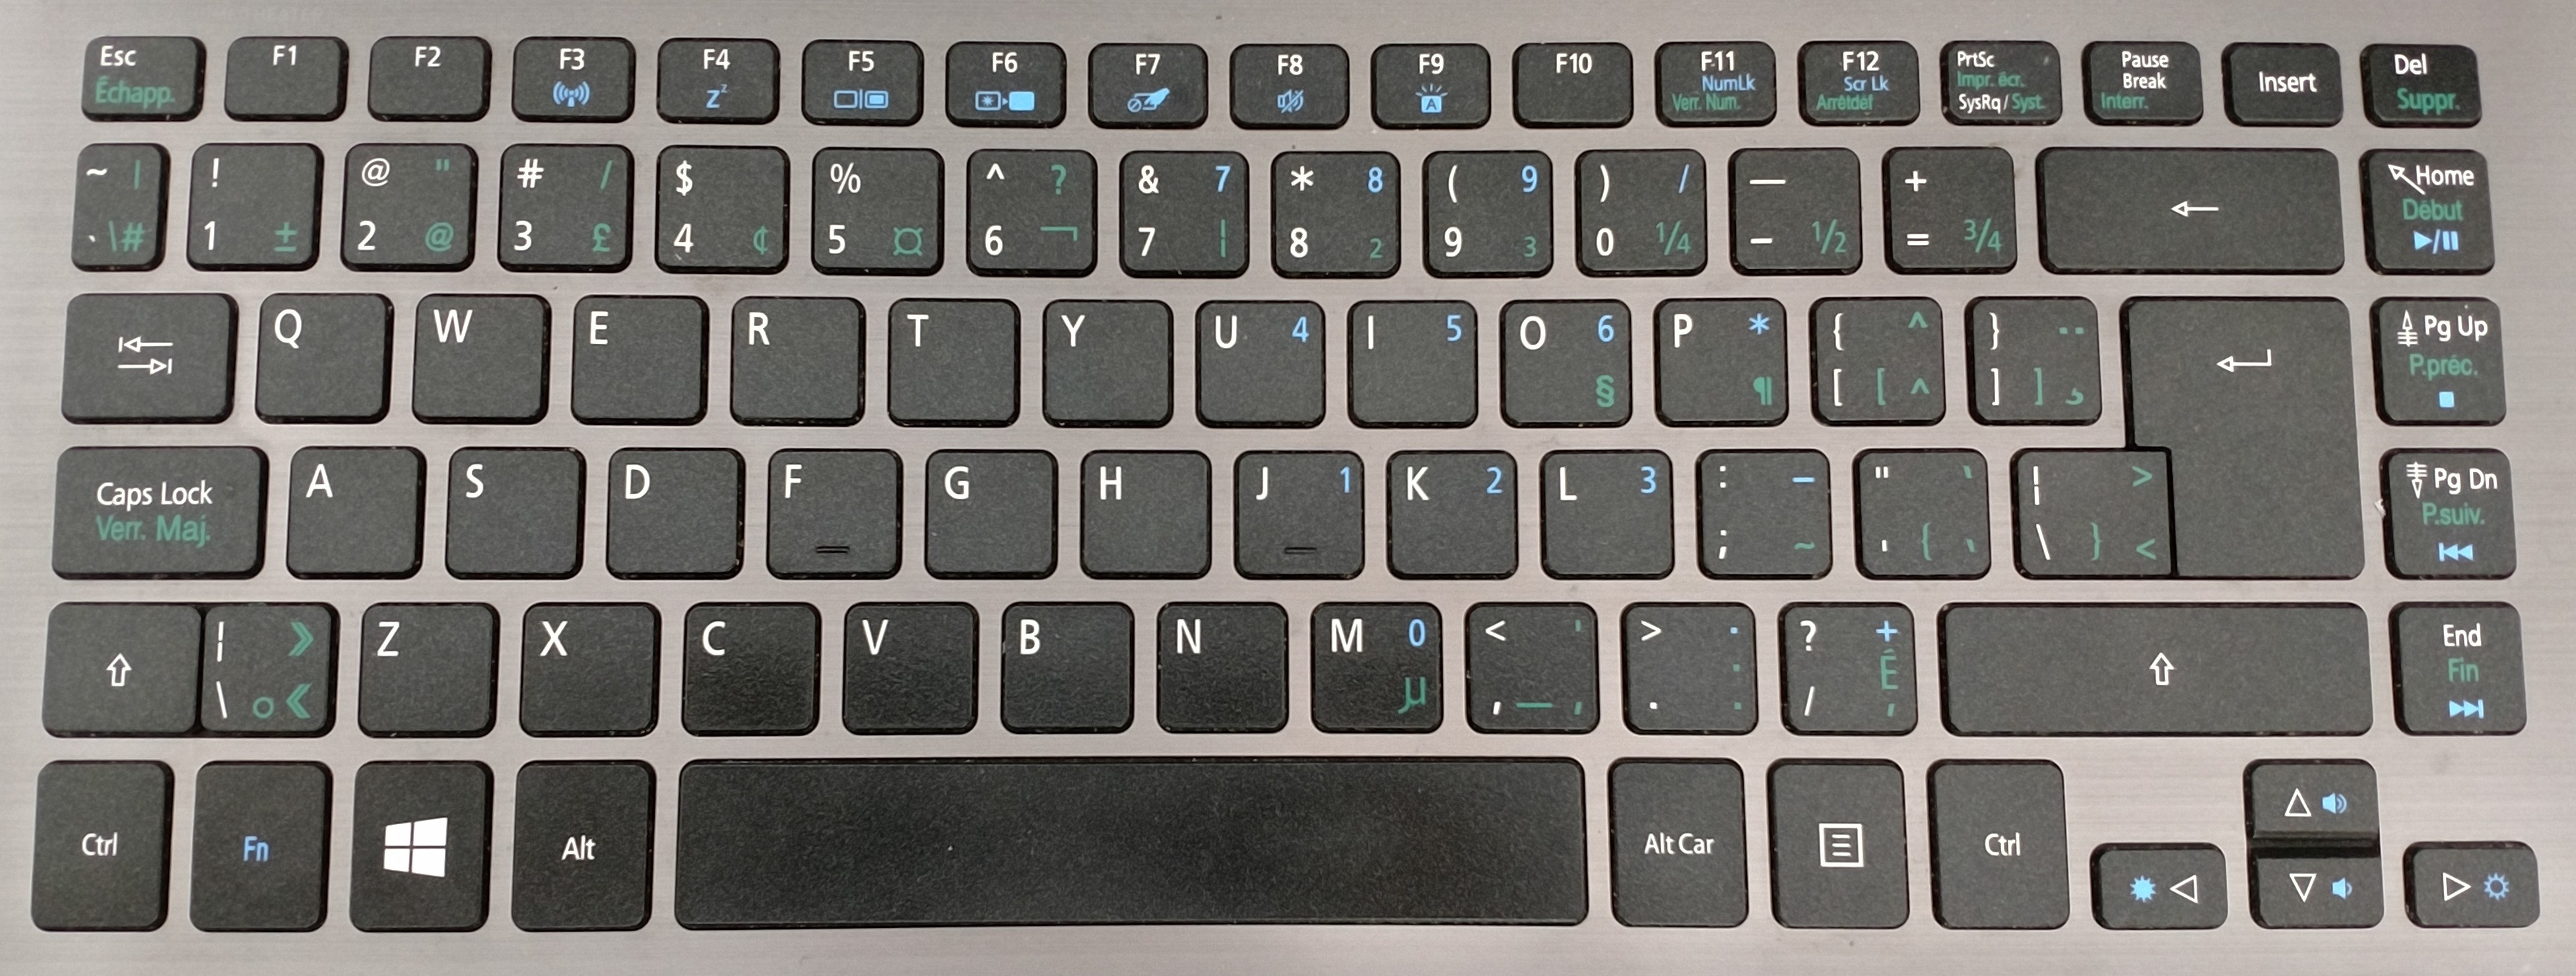
\includegraphics[height= 5cm]{Imagens/qwert.jpg}
	\label{f.qwert}
	\legend{\small Fonte: Elaborada pelo autor.}
\end{figure}

\citeonline{dix} descrevem os dispositivos de posicionamento e indicação dando o exemplo do mouse como um destes dispositivos. Outros dispositivos como os \textit{joysticks}, telas \textit{touchscreens}, \textit{touchpads} e as setas do teclado também estão nesta categoria.  Quando o contexto é um ambiente 3D, o mouse 3D, as luvas de dados (luvas com fibras ópticas ao longo dos dedos que detectam o ângulo das articulações) e capacetes de realidade virtual são alguns dos dispositivos desta categoria. 

Assim como os computadores \textit{desktops}, outros dispositivos de interação homem-máquina também tiveram a sua evolução ao longo do tempo. As telas \textit{touchscreens} sendo utilizadas como mouse em celulares e \textit{desktops}, o desenvolvimento de telas 3D e capacetes em realidade virtual capazes de criar ambientes imersivos são exemplos desta evolução. O crescimento dos dispositivos móveis acarretou no aumento do número de dispositivos de interação com estes minicomputadores como telas de alta densidade, capacidade gráfica 3D e sensores. Com a anexação de sensores como o acelerômetro e giroscópio foi possível a incorporação de aplicações em realidade virtual em dispositivos móveis.

\subsection{Acelerômetro e Giroscópio}
\label{ss.acelerometrogiroscopio}

Segundo \citeonline{bergstrom}, os sensores de inércia como os acelerômetros e os giroscópios possuem a função de converter um fenômeno físico em um sinal mensurável. O acelerômetro é normalmente definido num plano cartesiano e mede a força cinética causada por uma aceleração linear. Já os giroscópios medem a velocidade angular de uma rotação sob seu eixo primário.

De acordo com a empresa \citeonline{dimension}, a aceleração medida pelo acelerômetro pode ser estática ou dinâmica. A gravidade é um exemplo de força estática e uma das vantagens de medir esta aceleração é a possibilidade de descobrir o ângulo do dispositivo em relação à Terra. Já a medição da aceleração dinâmica revela em qual direção o dispositivo está se movendo. 

Quando inseridos em \textit{smartphones}, os acelerômetros podem ser utilizados para funções diversas que vão desde realizar a rotação da tela de acordo com a orientação em que o dispositivo se encontra até reconhecer movimentos do usuário como o caminhar e a movimentação da cabeça. 

Já os giroscópios funcionam como uma bússola indicando a posição do dispositivo no espaço. Estes medem a taxa de rotação ao longo dos três eixos do sensor, onde a rotação é positiva no sentido anti-horário. Aplicações em RV utilizam as informações do giroscópio para saber para onde o usuário está olhando através da rotação da cabeça. \cite{android}

\subsection{Computação Móvel}
\label{ss.computacaomovel}

Tendo em vista a popularidade e o avanço dos dispositivos móveis, é importante entender o significado de computação móvel a fim de se criar aplicações que podem ser executadas neste contexto. Para compreender o conceito de computação móvel, é preciso definir o que é mobilidade.

\begin{citacao}
	No contexto da computação móvel, mobilidade se refere ao uso pelas pessoas de dispositivos móveis portáveis funcionalmente poderosos que ofereçam a capacidade de realizar facilmente um conjunto de funções de aplicação, sendo também capazes de conectar-se, obter dados e fornecê-los a outros usuários, aplicações e sistemas. \cite[p. ~1]{lee}
\end{citacao}

Com os avanços do hardware dos computadores, foi possível criar aparelhos cada vez menores e, apesar dos dispositivos móveis serem portáteis, diferentes aparelhos possuem diferentes níveis de portabilidade. De acordo com \citeonline{lee}, a portabilidade é afetada pelos fatores tamanho e peso do dispositivo (considerando seus acessórios). Logo, um \textit{smartphone} que cabe em uma mão é mais portátil do que um laptop que necessita de uma bolsa ou maleta, por exemplo. 

Contudo, além da portabilidade também é necessário levar em consideração a usabilidade, a funcionalidade e a conectividade dos dispositivos. \citeonline{lee} definem a usabilidade como algo que depende do usuário, ambiente e as características do dispositivo enquanto que a funcionalidade é dividida nas categorias aplicações independentes, ou seja, o usuário não tem contato com outro usuário ou sistema, e dependentes (é necessário conectar-se a outro usuário ou sistema). Em relação à conectividade é importante apontar que um dispositivo móvel não possui necessariamente uma conexão sem fio.

Quanto à usabilidade é natural que um dispositivo móvel como um laptop seja mais facilmente transportado por um adulto do que por uma criança. Assim como certos usuários não possuem facilidade para interagir com certos dispositivos. Outros fatores como a característica do ambiente e as características do dispositivo afetam na escolha do dispositivo com melhor usabilidade. 

Em resumo, a computação móvel é definida a partir de diversos fatores. Diferentes tipos de dispositivos móveis possuem características distintas que, apesar de serem consideradas móveis, apresentam certas diferenças que devem ser levadas em consideração para se escolher o dispositivo mais adequado para determinada aplicação.

\textit{Smartphones} são dispositivos móveis que estão se tornando cada vez mais potentes. A evolução dos \textit{smartphones} permitiu a conexão de diversos dispositivos que aumentam ainda mais as possibilidades de interação homem-máquina. 

 	